%%%%%%%%%%%%%%%%%%%%%%%%%%%%%%%%%%%%%%%%%%%%%%%%%%%%%%%%%%%%%%%%%%%%%%%%%%%%%%%%%%
\begin{frame}[fragile]\frametitle{}
\begin{center}
{\Large Fine-tuning LLMs (Large Language Models)}
\end{center}
\end{frame}

%%%%%%%%%%%%%%%%%%%%%%%%%%%%%%%%%%%%%%%%%%%%%%%%%%%%%%%%%%%%%%%%%%%%%%%%%%%%%%%%%%
\begin{frame}[fragile]\frametitle{Introduction to Fine-Tuning}
  \begin{itemize}
      \item LLMs like GPT have vast language knowledge but lack specialization.
    \item Fine-tuning allows learning from domain-specific data for accuracy.
    \item \textbf{Definition:} Process of training pre-existing models on smaller, domain-specific datasets to enhance task or domain performance.

    \item \textbf{Example:} Healthcare organization fine-tunes on patient reports, adapting to medical terminologies.
	

	
	\item \textbf{Note}: Base Models are typically raw ie generic, may not give good results, but instruct-models are already tuned a bit, so they give better results. Fine-tuning either of them is ok, IMO. Instruct models come with their own prompt templates (read documentation).

    % \item \textbf{Applicability Beyond LLMs:} Fine-tuning for detecting trucks on highways.
  \end{itemize}
\end{frame}

%%%%%%%%%%%%%%%%%%%%%%%%%%%%%%%%%%%%%%%%%%%%%%%%%%%%%%%%%%%
\begin{frame}[fragile]\frametitle{See the Difference}


		\begin{center}
		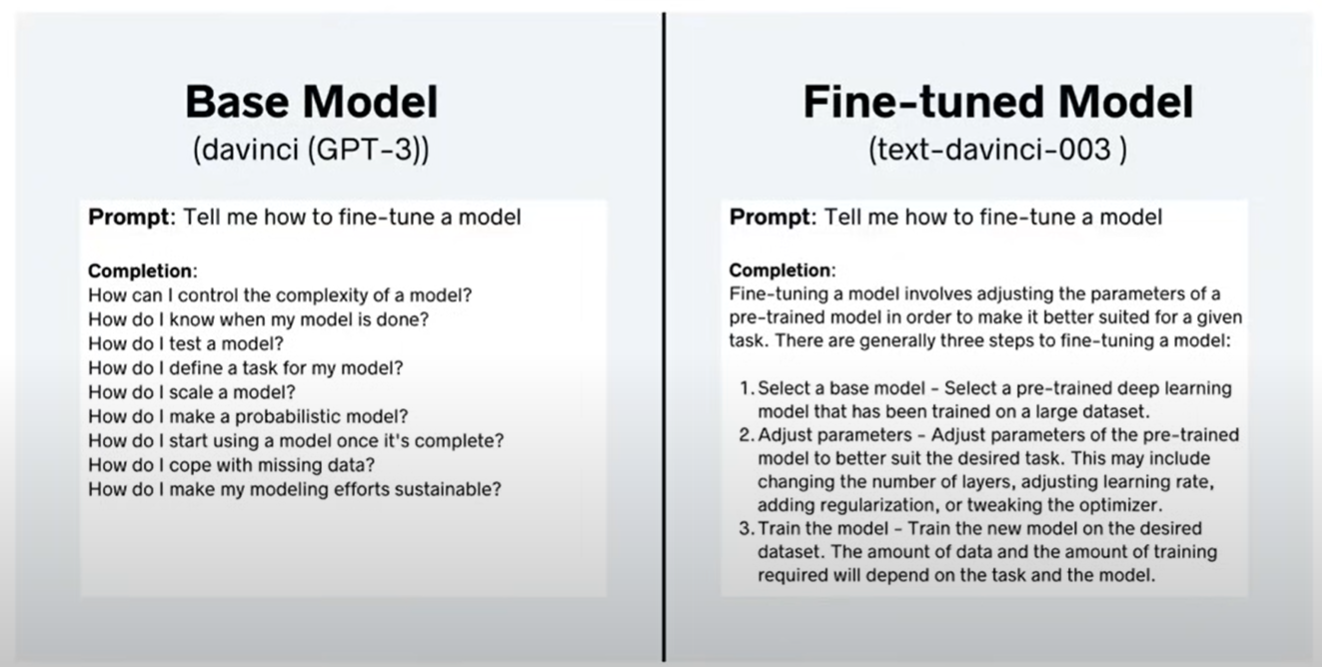
\includegraphics[width=\linewidth,keepaspectratio]{ft1}
		\end{center}

{\tiny (Ref: Fine-tuning Large Language Models (LLMs) | w/ Example Code - Shaw Talebi)}

\end{frame}



%%%%%%%%%%%%%%%%%%%%%%%%%%%%%%%%%%%%%%%%%%%%%%%%%%%%%%%%%%%%%%%%%%%%%%%%%%%%%%%%%%
\begin{frame}[fragile]\frametitle{Why? Customization}
  \begin{itemize}
    \item Each domain/task has unique language patterns, terminologies, nuances.
    \item Fine-tuning LLMs customizes them to understand domain-specific aspects.
    \item Customization aligns model's responses with specific requirements.
    \item Ensures accurate and contextually relevant outputs.
    \item LLMs excel in legal, medical, business, and other domains with specialized datasets.
    \item Fine-tuning empowers leveraging LLMs' power while maintaining accuracy.
  \end{itemize}
  
  {\tiny (ref: Fine-Tuning LLMs : Overview, Methods, and Best Practices - Turing)}
  
\end{frame}

%%%%%%%%%%%%%%%%%%%%%%%%%%%%%%%%%%%%%%%%%%%%%%%%%%%%%%%%%%%%%%%%%%%%%%%%%%%%%%%%%%
\begin{frame}[fragile]\frametitle{Why? Data compliance}
  \begin{itemize}
    \item Industries like healthcare, finance, law have strict data regulations.
    \item Fine-tuning LLMs on proprietary/regulated data ensures compliance.
    \item Develops LLMs trained specifically on in-house or industry data.
    \item Mitigates risk of exposing sensitive information to external models.
    \item Enhances security and privacy of data.
  \end{itemize}
  
  {\tiny (ref: Fine-Tuning LLMs : Overview, Methods, and Best Practices - Turing)}
  
\end{frame}

%%%%%%%%%%%%%%%%%%%%%%%%%%%%%%%%%%%%%%%%%%%%%%%%%%%%%%%%%%%%%%%%%%%%%%%%%%%%%%%%%%
\begin{frame}[fragile]\frametitle{Why? Limited labeled data}

  \begin{itemize}
    \item Obtaining labeled data for specific tasks/domains can be challenging.
    \item Fine-tuning adapts pre-trained LLM to available labeled dataset.
    \item Maximizes utility and performance of pre-existing labeled data.
    \item Overcomes constraints of data scarcity.
    \item Achieves significant improvements in model's accuracy and relevance.
  \end{itemize}
  
  {\tiny (ref: Fine-Tuning LLMs : Overview, Methods, and Best Practices - Turing)}
  
\end{frame}

% %%%%%%%%%%%%%%%%%%%%%%%%%%%%%%%%%%%%%%%%%%%%%%%%%%%%%%%%%%%%%%%%%%%%%%%%%%%%%%%%%%
% \begin{frame}[fragile]\frametitle{Why Fine-Tuning?}
  % \begin{itemize}
        % \item Large language models designed for versatility, not task mastery.
        % \item Fine-tuning essential for exceptional proficiency in specific tasks or domains.
        % \item Driven by the need for superior performance in targeted applications.
		% \item Through in-context learning or prompting, only a limited performance level is achievable.
		% \item Few-shot learning may not be effective for smaller LLMs. Consumes significant space in the context window.
  % \end{itemize}
% \end{frame}


% %%%%%%%%%%%%%%%%%%%%%%%%%%%%%%%%%%%%%%%%%%%%%%%%%%%%%%%%%%%%%%%%%%%%%%%%%%%%%%%%%%
% \begin{frame}[fragile]\frametitle{Why Fine-Tuning?}
    % \begin{itemize}
        % \item Pre-trained models are trained and built with general-purpose tasks, with Fine-tuning we can improve the performance of pre-trained models in wide range of domain-specific tasks.
        % \item Fine-tuning is a technique where a pre-trained model is trained on a new dataset.
		% \item Fine Tuning has many approaches, one uses adjusting last layer with retraining on custom data, another has adopter auxiliary network which gets trained on custom data, some have full retraining with frozen earlier weights.
		% \item Fine-tuning leverages a pre-trained model's knowledge and capabilities, saving significant time and resources compared to training a model from scratch. 
		% \item Improve factual response by utilizing Domain-specific data. 
		% \item Reduce Hallucinations.
    % \end{itemize}
% \end{frame}




% %%%%%%%%%%%%%%%%%%%%%%%%%%%%%%%%%%%%%%%%%%%%%%%%%%%%%%%%%%%%%%%%%%%%%%%%%%%%%%%%%%
% \begin{frame}[fragile]\frametitle{Why Fine-tuning?}
  % \begin{itemize}
    % \item \textbf{Domain-Specific Adaptation:}
      % \begin{itemize}
        % \item Pre-trained LLMs not optimized for specific tasks or domains.
        % \item Fine-tuning allows adaptation to nuances, enhancing performance.
        % \item Example: Fine-tuning for document analysis in the legal domain.
      % \end{itemize}
    % \item \textbf{Shifts in Data Distribution:}
      % \begin{itemize}
        % \item Models may not generalize well to out-of-distribution examples.
        % \item Fine-tuning aligns the model with new data distribution, improving performance.
        % \item Example: Fine-tuning a sentiment analysis model for social media comments.
      % \end{itemize}
    % \item \textbf{Cost and Resource Efficiency:}
      % \begin{itemize}
        % \item Training from scratch requires a large dataset, fine-tuning is more efficient.
        % \item Example: Adapting a pre-trained model for small e-commerce platform recommendations.
      % \end{itemize}
  % \end{itemize}
% \end{frame}

% %%%%%%%%%%%%%%%%%%%%%%%%%%%%%%%%%%%%%%%%%%%%%%%%%%%%%%%%%%%%%%%%%%%%%%%%%%%%%%%%%%
% \begin{frame}[fragile]\frametitle{Why Fine-tuning?}
  % \begin{itemize}
    % \item \textbf{Out-of-Distribution Data Handling:}
      % \begin{itemize}
        % \item Fine-tuning mitigates suboptimal performance with modest dataset.
        % \item Example: Fine-tuning a speech recognition model for a new regional accent.
      % \end{itemize}
    % \item \textbf{Knowledge Transfer:}
      % \begin{itemize}
        % \item Fine-tuning transfers general knowledge from pre-trained models to specific tasks.
        % \item Example: Transferring medical knowledge to a healthcare chatbot.
      % \end{itemize}
    % \item \textbf{Task-Specific Optimization:}
      % \begin{itemize}
        % \item Fine-tuning optimizes model parameters for specific task objectives.
        % \item Example: Optimizing a pre-trained model for code generation in software development.
      % \end{itemize}
  % \end{itemize}
% \end{frame}


% %%%%%%%%%%%%%%%%%%%%%%%%%%%%%%%%%%%%%%%%%%%%%%%%%%%%%%%%%%%%%%%%%%%%%%%%%%%%%%%%%%
% \begin{frame}[fragile]\frametitle{Why Fine-tuning?}
  % \begin{itemize}
    % \item \textbf{Adaptation to User Preferences:}
      % \begin{itemize}
        % \item Fine-tuning aligns the model with user preferences and task requirements.
        % \item Example: Fine-tuning a virtual assistant model for user-specific language and tone.
      % \end{itemize}
    % \item \textbf{Continual Learning:}
      % \begin{itemize}
        % \item Fine-tuning supports continual learning, adapting to evolving data and user needs.
        % \item Example: Continually updating a news summarization model for evolving news topics.
      % \end{itemize}
  % \end{itemize}
% \end{frame}

%%%%%%%%%%%%%%%%%%%%%%%%%%%%%%%%%%%%%%%%%%%%%%%%%%%%%%%%%%%%%%%%%%%%%%%%%%%%%%%%%%
\begin{frame}[fragile]\frametitle{How? Last layer, Feature extraction (repurposing)}

  \begin{itemize}
    \item Feature extraction (repurposing) is a primary approach for fine-tuning LLMs.
    \item Pre-trained LLM treated as fixed feature extractor.
    \item Model learns significant language features from vast dataset.
    \item Final layers trained on task-specific data while rest of model remains frozen.
    \item Leverages rich representations learned by LLM, adapting them to specific task.
    \item Offers cost-effective and efficient fine-tuning.
  \end{itemize}
  
  {\tiny (ref: Fine-Tuning LLMs : Overview, Methods, and Best Practices - Turing)}
  
\end{frame}

%%%%%%%%%%%%%%%%%%%%%%%%%%%%%%%%%%%%%%%%%%%%%%%%%%%%%%%%%%%%%%%%%%%%%%%%%%%%%%%%%%
\begin{frame}[fragile]\frametitle{How? Full fine-tuning}

  \begin{itemize}
    \item Full fine-tuning is another primary approach for LLM fine-tuning.
    \item Differs from feature extraction by training entire model on task-specific data.
    \item All model layers adjusted during training.
    \item Particularly beneficial for large, significantly different task-specific datasets.
    \item Allows deeper adaptation of model to specific task.
    \item May lead to superior performance but requires more computational resources and time.
  \end{itemize}
  
  {\tiny (ref: Fine-Tuning LLMs : Overview, Methods, and Best Practices - Turing)}
  
\end{frame}

% %%%%%%%%%%%%%%%%%%%%%%%%%%%%%%%%%%%%%%%%%%%%%%%%%%%%%%%%%%%
% \begin{frame}[fragile]\frametitle{How? Supervised fine-tuning}


% \begin{itemize}
  % \item Supervised learning process adjusting LLM/Adapter weights.
  % \item Uses a labeled dataset of prompt-completion pairs.
  % \item Types:
  % \begin{itemize}
	  % \item \textbf{Instruction Fine Tuning:}
		% \begin{itemize}
		  % \item Trains LLM on examples of instructions and desired responses.
		  % \item Improves performance on instruction-specific tasks.
		% \end{itemize}

	  % \item \textbf{Full Fine Tuning:}
		% \begin{itemize}
		  % \item Updates all LLM parameters.
		  % \item Requires sufficient memory for storing and processing gradients and components.
		% \end{itemize}
  % \end{itemize}

% \end{itemize}


% {\tiny (Ref: Generative AI with Large Language Model - Abhinav  Kimothi)}

% \end{frame}

%%%%%%%%%%%%%%%%%%%%%%%%%%%%%%%%%%%%%%%%%%%%%%%%%%%%%%%%%%%
\begin{frame}[fragile]\frametitle{What is a fine-tuned LLM?}


		\begin{center}
		\includegraphics[width=\linewidth,keepaspectratio]{rag8}
		\end{center}

{\tiny (Ref: Generative AI with Large Language Model - Abhinav  Kimothi)}

\end{frame}


% %%%%%%%%%%%%%%%%%%%%%%%%%%%%%%%%%%%%%%%%%%%%%%%%%%%%%%%%%%%
% \begin{frame}[fragile]\frametitle{Ways to fine-tune}


		% \begin{center}
		% \includegraphics[width=\linewidth,keepaspectratio]{finetune7}
		% \end{center}

% {\tiny (Ref: Fine-tuning Large Language Models (LLMs) | w/ Example Code - Shaw Talebi)}

% \end{frame}

%%%%%%%%%%%%%%%%%%%%%%%%%%%%%%%%%%%%%%%%%%%%%%%%%%%%%%%%%%%
\begin{frame}[fragile]\frametitle{Ways to change parameters/weights}


		\begin{center}
		\includegraphics[width=\linewidth,keepaspectratio]{finetune8}
		\end{center}

{\tiny (Ref: Fine-tuning Large Language Models (LLMs) | w/ Example Code - Shaw Talebi)}

\end{frame}


% %%%%%%%%%%%%%%%%%%%%%%%%%%%%%%%%%%%%%%%%%%%%%%%%%%%%%%%%%%%%%%%%%%%%%%%%%%%%%%%%%%
% \begin{frame}[fragile]\frametitle{Task specific Fine-Tuning}
    % \begin{itemize}
        % \item Widely used for customizing pre-trained LLMs to specific tasks.
        % \item Involves training on labeled prompt-completion pairs.
        % \item Allows model to adjust weights for task alignment.
    % \end{itemize}
% \end{frame}

% %%%%%%%%%%%%%%%%%%%%%%%%%%%%%%%%%%%%%%%%%%%%%%%%%%%%%%%%%%%%%%%%%%%%%%%%%%%%%%%%%%
% \begin{frame}[fragile]\frametitle{Unsupervised Fine-Tuning Methods}

% \begin{itemize}
% \item \textbf{Unsupervised Full Fine-Tuning:}
  % \begin{itemize}
	% \item Relevant for updating LLM knowledge base without changing existing behavior.
	% \item Example: Fine-tuning on legal literature or adapting to a new language using unstructured datasets.
  % \end{itemize}
% \item \textbf{Contrastive Learning:}
  % \begin{itemize}
	% \item Trains the model to discern between similar and dissimilar examples in the latent space.
	% \item Beneficial for tasks requiring nuanced understanding of similarities and distinctions.
  % \end{itemize}
% \end{itemize}
% \end{frame}

%%%%%%%%%%%%%%%%%%%%%%%%%%%%%%%%%%%%%%%%%%%%%%%%%%%%%%%%%%%%%%%%%%%%%%%%%%%%%%%%%%
\begin{frame}[fragile]\frametitle{Fine-Tuning Methods}

\begin{itemize}
\item \textbf{Supervised Full Fine-Tuning:}
  \begin{itemize}
	\item Involves updating all parameters of the language model during training.
	\item Resource-intensive but ensures thorough adaptation of the entire model to the task or domain.
  \end{itemize}
\item \textbf{Instruction Fine-Tuning:}
  \begin{itemize}
	\item Involves training the model using examples with explicit instructions for specific queries or tasks.
	\item Suitable for applications where precise task execution is essential.
  \end{itemize}
\item \textbf{Reinforcement Learning from Human Feedback (RLHF):}
  \begin{itemize}
	\item Incorporates reinforcement learning principles with human evaluators providing ratings.
	\item Ratings serve as rewards, guiding the model to optimize parameters based on human preferences.
  \end{itemize}
\item \textbf{Parameter-Efficient Fine-Tuning (PEFT):}
  \begin{itemize}
	\item Aims to reduce computational expenses by selectively updating a small set of parameters.
	\item Example: Low-rank adaptation (LoRA) technique focuses on updating only relevant parameters.
  \end{itemize}  
\end{itemize}

\end{frame}

% %%%%%%%%%%%%%%%%%%%%%%%%%%%%%%%%%%%%%%%%%%%%%%%%%%%%%%%%%%%%%%%%%%%%%%%%%%%%%%%%%%
% \begin{frame}[fragile]\frametitle{Instruction Fine-Tuning}
  % \begin{itemize}
    % \item \textbf{Overview:}
      % \begin{itemize}
        % \item Instruction fine-tuning enhances LLMs for real-world applications.
        % \item Differs from standard supervised fine-tuning by augmenting examples with explicit instructions.
        % \item Instruction-tuned models generalize effectively to new tasks, providing additional context.
      % \end{itemize}
    % \item \textbf{Value in NLP and ML:}
      % \begin{itemize}
        % \item Instruction fine-tuning is crucial in the evolving landscape of NLP and ML.
        % \item Enables LLMs to adapt to specific tasks with nuanced instructions.
      % \end{itemize}	  
  % \end{itemize}

% \begin{center}
% \includegraphics[width=\linewidth,keepaspectratio]{llm128}
% \end{center}				

% {\tiny (Ref: Applied LLMs Mastery 2024 - Aishwarya Reganti)}

% \end{frame}


% %%%%%%%%%%%%%%%%%%%%%%%%%%%%%%%%%%%%%%%%%%%%%%%%%%%%%%%%%%%%%%%%%%%%%%%%%%%%%%%%%%
% \begin{frame}[fragile]\frametitle{Example: Natural Instructions Dataset}
  % \begin{itemize}
    % \item \textbf{Dataset Overview:}
      % \begin{itemize}
        % \item "Natural Instructions" dataset consists of 193,000 instruction-output examples.
        % \item Sourced from 61 existing English NLP tasks.
        % \item Structured approach with crowd-sourced instructions aligned to a common schema.
      % \end{itemize}
    % \item \textbf{Unique Features:}
      % \begin{itemize}
        % \item Each instruction associated with a task, providing explicit guidance for the model.
        % \item Covers fields like definition, things to avoid, positive and negative examples.
        % \item Structured nature makes it valuable for fine-tuning, offering clear and detailed instructions.
      % \end{itemize}
  % \end{itemize}
% \end{frame}


% %%%%%%%%%%%%%%%%%%%%%%%%%%%%%%%%%%%%%%%%%%%%%%%%%%%%%%%%%%%%%%%%%%%%%%%%%%%%%%%%%%
% \begin{frame}[fragile]\frametitle{Example: Natural Instructions Dataset}

% \begin{center}
% \includegraphics[width=\linewidth,keepaspectratio]{llm129}
% \end{center}				

% {\tiny (Ref: Applied LLMs Mastery 2024 - Aishwarya Reganti)}

% \end{frame}

% %%%%%%%%%%%%%%%%%%%%%%%%%%%%%%%%%%%%%%%%%%%%%%%%%%%%%%%%%%%%%%%%%%%%%%%%%%%%%%%%%%
% \begin{frame}[fragile]\frametitle{Leveraging Instruction Fine-Tuning}
    % \begin{itemize}
        % \item Extension of traditional fine-tuning.
        % \item Trains model on examples of instructions and desired responses.
        % \item Offers improved interpretability, controlled outputs, and reduced biases.
        % \item Enables explicit task specification learning for enhanced performance.
    % \end{itemize}
% \end{frame}

% %%%%%%%%%%%%%%%%%%%%%%%%%%%%%%%%%%%%%%%%%%%%%%%%%%%%%%%%%%%%%%%%%%%%%%%%%%%%%%%%%%
% \begin{frame}[fragile]\frametitle{Full Fine-Tuning Potential}
    % \begin{itemize}
        % \item Updates all parameters of the language model during training.
        % \item Enhances adaptability to specific tasks for potentially better performance.
        % \item Demands significant memory for processing gradients and other components.
        % \item Challenging to implement on resource-constrained devices or environments.
    % \end{itemize}
% \end{frame}

% %%%%%%%%%%%%%%%%%%%%%%%%%%%%%%%%%%%%%%%%%%%%%%%%%%%%%%%%%%%%%%%%%%%%%%%%%%%%%%%%%%
% \begin{frame}[fragile]\frametitle{Reinforcement Learning from Human Feedback (RLHF)}
  % \begin{itemize}
        % \item RLHF enhances language models by incorporating human feedback.
        % \item Aims to align models more closely with intricate human values.
  % \end{itemize}
  
% \begin{center}
% \includegraphics[width=0.8\linewidth,keepaspectratio]{llm130}
% \end{center}				

% {\tiny (Ref: Applied LLMs Mastery 2024 - Aishwarya Reganti)}  
% \end{frame}

% %%%%%%%%%%%%%%%%%%%%%%%%%%%%%%%%%%%%%%%%%%%%%%%%%%%%%%%%%%%%%%%%%%%%%%%%%%%%%%%%%%
% \begin{frame}[fragile]\frametitle{RLHF Process - Step 1}
  % \begin{itemize}
    % \item \textbf{Pretraining Language Models (LMs):}
      % \begin{itemize}
        % \item RLHF starts with a pretrained LM, typically achieved through classical pretraining objectives.
        % \item Initial LM, flexible in size, can undergo optional fine-tuning on additional data.
        % \item Crucial to have a model with positive response to diverse instructions.
      % \end{itemize}
  % \end{itemize}
% \end{frame}

% %%%%%%%%%%%%%%%%%%%%%%%%%%%%%%%%%%%%%%%%%%%%%%%%%%%%%%%%%%%%%%%%%%%%%%%%%%%%%%%%%%
% \begin{frame}[fragile]\frametitle{RLHF Process - Step 2}
  % \begin{itemize}
    % \item \textbf{Reward Model Training:}
      % \begin{itemize}
        % \item Involves generating a reward model (RM) calibrated with human preferences.
        % \item RM assigns scalar rewards to text sequences, reflecting human preferences.
        % \item Dataset for training RM generated by sampling prompts, passing through initial LM, and ranking by human annotators.
        % \item Reward function combines preference model and a penalty on RL policy vs. initial model difference.
      % \end{itemize}
  % \end{itemize}
% \end{frame}

% %%%%%%%%%%%%%%%%%%%%%%%%%%%%%%%%%%%%%%%%%%%%%%%%%%%%%%%%%%%%%%%%%%%%%%%%%%%%%%%%%%
% \begin{frame}[fragile]\frametitle{RLHF Process - Step 3}
  % \begin{itemize}
    % \item \textbf{Fine-Tuning with RL:}
      % \begin{itemize}
        % \item Final step involves fine-tuning the initial LLM using reinforcement learning.
        % \item Proximal Policy Optimization (PPO) commonly used for RL algorithm.
        % \item RL policy is LM that takes prompt, produces text, with actions corresponding to tokens in LM's vocabulary.
        % \item PPO updates LM's parameters to maximize reward metrics, aligning model with human preferences.
        % \item Some parameters frozen due to computational constraints.
      % \end{itemize}
  % \end{itemize}
% \end{frame}

% %%%%%%%%%%%%%%%%%%%%%%%%%%%%%%%%%%%%%%%%%%%%%%%%%%%%%%%%%%%%%%%%%%%%%%%%%%%%%%%%%%
% \begin{frame}[fragile]\frametitle{Direct Preference Optimization (DPO)}
  % \begin{itemize}
    % \item \textbf{Overview:}
      % \begin{itemize}
        % \item DPO is equivalent to RLHF and gaining significant traction.
        % \item Offers a straightforward method for fine-tuning large language models based on human preferences.
        % \item Eliminates the need for a complex reward model, directly incorporating user feedback into the optimization process.
      % \end{itemize}
    % \item \textbf{User-Friendly Approach:}
      % \begin{itemize}
        % \item Users compare two model-generated outputs and express preferences.
        % \item LLM adjusts its behavior accordingly, simplifying the optimization process.
        % \item Advantages include ease of implementation, computational efficiency, and greater control over LLM's behavior.
      % \end{itemize}
  % \end{itemize}

% \begin{center}
% \includegraphics[width=\linewidth,keepaspectratio]{llm131}
% \end{center}				

% {\tiny (Ref: Applied LLMs Mastery 2024 - Aishwarya Reganti)}

% \end{frame}


% %%%%%%%%%%%%%%%%%%%%%%%%%%%%%%%%%%%%%%%%%%%%%%%%%%%%%%%%%%%%%%%%%%%%%%%%%%%%%%%%%%
% \begin{frame}[fragile]\frametitle{Comparison: DPO vs RLHF}
  % \begin{itemize}
    % \item \textbf{DPO Approach:}
      % \begin{itemize}
        % \item Directly optimizes LM based on user preferences without a separate reward model.
        % \item Users compare two model-generated outputs to guide the optimization process.
      % \end{itemize}

    % \item \textbf{Maximum Likelihood in LLM Training:}
      % \begin{itemize}
        % \item Maximum likelihood is a principle used during LLM training.
        % \item Involves adjusting model's parameters to maximize the likelihood of generating actual sequences observed in training data.
        % \item Helps LLM learn to generate text similar to examples it was trained on.
      % \end{itemize}
    % \item \textbf{RLHF Approach:}
      % \begin{itemize}
        % \item Follows a more structured path, leveraging reinforcement learning principles.
        % \item Involves training a reward model to identify and reward desirable LM outputs.
        % \item Reward model guides LM's training process, shaping its behavior towards positive outcomes.
      % \end{itemize}
    % \item \textbf{DPO - A Simpler Approach:}
      % \begin{itemize}
        % \item Direct Policy Optimization (DPO) takes a straightforward path.
        % \item Sidesteps the need for a complex reward model in fine-tuning Large Language Models (LLMs).
        % \item Optimizes LLM directly based on user preferences by comparing two outputs.
      % \end{itemize}
  % \end{itemize}
% \end{frame}

% %%%%%%%%%%%%%%%%%%%%%%%%%%%%%%%%%%%%%%%%%%%%%%%%%%%%%%%%%%%%%%%%%%%%%%%%%%%%%%%%%%
% \begin{frame}[fragile]\frametitle{DPO Advantages}
  % \begin{itemize}
    % \item \textbf{Ease of Implementation:}
      % \begin{itemize}
        % \item DPO is more user-friendly, eliminating the need for a separate reward model.
        % \item Accessible to a broader audience due to its simplicity.
      % \end{itemize}
    % \item \textbf{Computational Efficiency:}
      % \begin{itemize}
        % \item Operates directly on the LLM, leading to faster training times.
        % \item Lower computational costs compared to RLHF.
      % \end{itemize}
    % \item \textbf{Greater Control:}
      % \begin{itemize}
        % \item Users have direct control over LLM's behavior without complexities.
        % \item Enables guidance toward specific goals and preferences.
      % \end{itemize}
    % \item \textbf{Faster Convergence:}
      % \begin{itemize}
        % \item Due to its simpler structure and direct optimization, DPO often achieves faster results.
        % \item Suitable for tasks with rapid iteration needs.
      % \end{itemize}
    % \item \textbf{Improved Performance:}
      % \begin{itemize}
        % \item Recent research suggests DPO can outperform RLHF in sentiment control and response quality.
        % \item Particularly effective in summarization and dialogue tasks.
      % \end{itemize}
  % \end{itemize}
% \end{frame}

% %%%%%%%%%%%%%%%%%%%%%%%%%%%%%%%%%%%%%%%%%%%%%%%%%%%%%%%%%%%%%%%%%%%%%%%%%%%%%%%%%%
% \begin{frame}[fragile]\frametitle{RLHF - A More Structured Approach}
  % \begin{itemize}
    % \item \textbf{More Structured Path:}
      % \begin{itemize}
        % \item Reinforcement Learning from Human Feedback (RLHF) follows a more structured path.
        % \item Leverages reinforcement learning principles in three training phases.
      % \end{itemize}
    % \item \textbf{Complexity:}
      % \begin{itemize}
        % \item RLHF can be more complex and sometimes unstable.
        % \item Demands more computational resources and deals with convergence, drift, or uncorrelated distribution problems.
      % \end{itemize}
    % \item \textbf{Flexibility in Defining Rewards:}
      % \begin{itemize}
        % \item RLHF allows more nuanced reward structures, beneficial for precise control over LLM's output.
      % \end{itemize}
    % \item \textbf{Handling Diverse Feedback Formats:}
      % \begin{itemize}
        % \item RLHF can handle various forms of human feedback, including numerical ratings or textual corrections.
        % \item DPO primarily relies on binary preferences for user feedback.
      % \end{itemize}
    % \item \textbf{Handling Large Datasets:}
      % \begin{itemize}
        % \item RLHF can be more efficient in handling massive datasets, especially with distributed training techniques.
      % \end{itemize}
  % \end{itemize}
% \end{frame}

% %%%%%%%%%%%%%%%%%%%%%%%%%%%%%%%%%%%%%%%%%%%%%%%%%%%%%%%%%%%%%%%%%%%%%%%%%%%%%%%%%%
% \begin{frame}[fragile]\frametitle{Summary: PPO vs DPO}
  % \begin{itemize}
    % \item \textbf{Choice Depends On:}
      % \begin{itemize}
        % \item Specific task requirements.
        % \item Available computational resources.
        % \item Desired level of control over LLM's behavior.
      % \end{itemize}
    % \item \textbf{Strengths and Weaknesses:}
      % \begin{itemize}
        % \item Both methods offer strengths and weaknesses in different contexts.
        % \item Evolving and enhancing fine-tuning processes for LLMs.
      % \end{itemize}
  % \end{itemize}
% \end{frame}

%%%%%%%%%%%%%%%%%%%%%%%%%%%%%%%%%%%%%%%%%%%%%%%%%%%%%%%%%%%%%%%%%%%%%%%%%%%%%%%%%%
\begin{frame}[fragile]\frametitle{}
\begin{center}
{\Large Parameter Efficient Fine Tuning (PEFT)}
\end{center}
\end{frame}

% %%%%%%%%%%%%%%%%%%%%%%%%%%%%%%%%%%%%%%%%%%%%%%%%%%%%%%%%%%%%%%%%%%%%%%%%%%%%%%%%%%
% \begin{frame}[fragile]\frametitle{Introduction}

  % \begin{itemize}
    % \item Form of instruction fine-tuning, more efficient than full fine-tuning.
    % \item Full LLM fine-tuning demands significant computational resources.
    % \item PEFT updates only subset of parameters, "freezing" the rest.
    % \item Reduces trainable parameters, making memory requirements manageable.
    % \item Prevents catastrophic forgetting.
    % \item Maintains original LLM weights, avoids loss of previously learned information.
    % \item Beneficial for handling storage issues when fine-tuning for multiple tasks.
	% \item Methods for Parameter Efficient Fine-Tuning: Low-Rank Adaptation (LoRA) and QLoRA
  % \end{itemize}
  
  % {\tiny (ref: Fine-Tuning LLMs : Overview, Methods, and Best Practices - Turing)}
  
% \end{frame}


%%%%%%%%%%%%%%%%%%%%%%%%%%%%%%%%%%%%%%%%%%%%%%%%%%%%%%%%%%%
\begin{frame}[fragile]\frametitle{What PEFT addresses?}

\begin{itemize}
  \item \textbf{Full Fine Tuning:}
    \begin{itemize}
      \item Requires memory for the entire model, optimizers, gradients, etc.
      \item Similar memory demands as pre-training.
    \end{itemize}

  \item \textbf{Parameter-Efficient Fine Tuning (PEFT):}
    \begin{itemize}
      \item Fine-tunes only a subset of model parameters.
      \item In some cases, leaves the original weights untouched.
    \end{itemize}
	
    \item \textbf{Addressing Resource Intensity:}
      \begin{itemize}
        \item PEFT addresses the resource-intensive nature of fine-tuning Large Language Models (LLMs).
        \item Full fine-tuning modifies all parameters, while PEFT fine-tunes only a small subset, minimizing computational demands.
      \end{itemize}	
\end{itemize}

PEFT is a library from Hugging Face which comes with several options to train models efficiently, one of them is LoRA.

{\tiny (Ref: Generative AI with Large Language Model - Abhinav  Kimothi)}

\end{frame}


%%%%%%%%%%%%%%%%%%%%%%%%%%%%%%%%%%%%%%%%%%%%%%%%%%%%%%%%%%%
\begin{frame}[fragile]\frametitle{What is Parameter Efficient Fine Tuning?}


		\begin{center}
		\includegraphics[width=0.8\linewidth,keepaspectratio]{rag9}
		\end{center}

{\tiny (Ref: Generative AI with Large Language Model - Abhinav  Kimothi)}

\end{frame}




% %%%%%%%%%%%%%%%%%%%%%%%%%%%%%%%%%%%%%%%%%%%%%%%%%%%%%%%%%%%
% \begin{frame}[fragile]\frametitle{Compute Memory Optimization in LLM training : FSDP}

% \begin{itemize}
  % \item \textbf{Resource Intensive Training:}
    % \begin{itemize}
      % \item Training large language models demands substantial computational resources and time.
      % \item Due to the vast size and complexity of these models.
    % \end{itemize}

  % \item \textbf{Fully Sharded Data Parallelism (FSDP):}
    % \begin{itemize}
      % \item Efficiently distributes training workload across multiple machines or processors.
      % \item Enables faster and more scalable training.
    % \end{itemize}

  % \item \textbf{Comprehensive Approach:}
    % \begin{itemize}
      % \item FSDP handles both data and model parameters, enhancing overall efficiency.
      % \item Reduces communication overhead during training.
    % \end{itemize}

  % \item \textbf{Communication Overhead Reduction:}
    % \begin{itemize}
      % \item Achieved by partitioning model parameters into shards.
      % \item Minimizes information exchange between devices during training.
    % \end{itemize}

  % \item \textbf{Hardware Flexibility:}
    % \begin{itemize}
      % \item FSDP supports a mix of GPUs, TPUs, or other specialized hardware in training clusters.
    % \end{itemize}
% \end{itemize}

% {\tiny (Ref: Generative AI with Large Language Model - Abhinav  Kimothi)}

% \end{frame}


% %%%%%%%%%%%%%%%%%%%%%%%%%%%%%%%%%%%%%%%%%%%%%%%%%%%%%%%%%%%
% \begin{frame}[fragile]\frametitle{Compute Memory Optimisation in LLM training : FSDP}


		% \begin{center}
		% \includegraphics[width=\linewidth,keepaspectratio]{rag10}
		% \end{center}

% {\tiny (Ref: Generative AI with Large Language Model - Abhinav  Kimothi)}

% \end{frame}



% %%%%%%%%%%%%%%%%%%%%%%%%%%%%%%%%%%%%%%%%%%%%%%%%%%%%%%%%%%%
% \begin{frame}[fragile]\frametitle{Can, Cannot}

% Over time, LLMs will improve in:
% \begin{itemize}
% \item Better instructions following
% \item Large Contexts
% \item Simple strategies to fine tune
% \end{itemize}	

% But, LLMs will not improve in:
% \begin{itemize}
% \item Information Extraction/retrieval: cant have real time data access, not 100\% trustworthy
% \end{itemize}

% Need knowledge base support

% {\tiny (Ref: Combining LLMs with Knowledge Bases to Prevent Hallucinations - Scott Mackie - LLMs in Prod Con 2 )}

% \end{frame}

% %%%%%%%%%%%%%%%%%%%%%%%%%%%%%%%%%%%%%%%%%%%%%%%%%%%%%%%%%%%
% \begin{frame}[fragile]\frametitle{Adding support of Knowledge Base}

% To prevent hallucinations. The paper suggested is wrong.


% \begin{center}
% \includegraphics[width=\linewidth,keepaspectratio]{llm59}
% \end{center}		


% {\tiny (Ref: Combining LLMs with Knowledge Bases to Prevent Hallucinations - Scott Mackie - LLMs in Prod Con 2 )}

% \end{frame}

% %%%%%%%%%%%%%%%%%%%%%%%%%%%%%%%%%%%%%%%%%%%%%%%%%%%%%%%%%%%
% \begin{frame}[fragile]\frametitle{Part I: Access to Knowledge Base}

% \begin{center}
% \includegraphics[width=\linewidth,keepaspectratio]{llm60}
% \end{center}		


% {\tiny (Ref: Combining LLMs with Knowledge Bases to Prevent Hallucinations - Scott Mackie - LLMs in Prod Con 2 )}

% \end{frame}

% %%%%%%%%%%%%%%%%%%%%%%%%%%%%%%%%%%%%%%%%%%%%%%%%%%%%%%%%%%%
% \begin{frame}[fragile]\frametitle{Part II: Add Guardrails}

% to have only answers that are grounded. Dont ask maths!!

% \begin{center}
% \includegraphics[width=\linewidth,keepaspectratio]{llm61}
% \end{center}		


% {\tiny (Ref: Combining LLMs with Knowledge Bases to Prevent Hallucinations - Scott Mackie - LLMs in Prod Con 2 )}

% \end{frame}



% %%%%%%%%%%%%%%%%%%%%%%%%%%%%%%%%%%%%%%%%%%%%%%%%%%%%%%%%%%%
% \begin{frame}[fragile]\frametitle{Prompt Engineering}

% \begin{itemize}
% \item technique to tweak the input so that the output matches your expectations. 
% \item provide some examples of the expected output format. 
% \item similar to a zero-shot or few-shot learning setting
% \end{itemize}	

% \begin{center}
% \includegraphics[width=\linewidth,keepaspectratio]{promptengg30}
% \end{center}		

% {\tiny (Ref: Understanding LLMOps: Large Language Model Operations by Leonie )}

% \end{frame}



% %%%%%%%%%%%%%%%%%%%%%%%%%%%%%%%%%%%%%%%%%%%%%%%%%%%%%%%%%%%
% \begin{frame}[fragile]\frametitle{Fine-tuning LLMs}

% \begin{itemize}
% \item help improve your model's performance on your specific task. 
% \item Although this will increase the training efforts, it can reduce the cost of inference. 
% \item The cost of LLM APIs is dependent on input and output sequence length. 
% \item Thus, reducing the number of input tokens, reduces API costs because you don't have to provide examples in the prompt anymore
% \end{itemize}	

% \begin{center}
% \includegraphics[width=0.8\linewidth,keepaspectratio]{promptengg31}
% \end{center}		

% {\tiny (Ref: Understanding LLMOps: Large Language Model Operations by Leonie )}

% \end{frame}

% %%%%%%%%%%%%%%%%%%%%%%%%%%%%%%%%%%%%%%%%%%%%%%%%%%%%%%%%%%%
% \begin{frame}[fragile]\frametitle{Fine-tuning LLMs}

% \begin{center}
% \includegraphics[width=0.8\linewidth,keepaspectratio]{langchain6}

% {\tiny (Ref: FutureSmart AI Blog)}

% \end{center}		


% \end{frame}

% %%%%%%%%%%%%%%%%%%%%%%%%%%%%%%%%%%%%%%%%%%%%%%%%%%%%%%%%%%%
% \begin{frame}[fragile]\frametitle{5 tips Fine-tuning GPT}

% \begin{itemize}
% \item Start with normal gpt 3 and prompt engineering, make max progress possible. If that suffices, well and good. Its powerful. Language used in Prompt Engineering matters
% \item Data gathering for Fine Tuning is far more laboursome than Prompt Engineering.
% \item Have separation between the context and query not just with 3 hashes but with some phrase like, ''here are the questions''.
% \item Use GPT 3 itself to generate synthetic datasets. Small fine-tuning data is good enough.
% \item Fine tuning improves consistency at the cost of creativity
% \end{itemize}	

% {\tiny (Ref: 5 Tips and Misconceptions about Finetuning GPT-3 - David Shapiro AI)}


% \end{frame}

%%%%%%%%%%%%%%%%%%%%%%%%%%%%%%%%%%%%%%%%%%%%%%%%%%%%%%%%%%%%%%%%%%%%%%%%%%%%%%%%%%
\begin{frame}[fragile]\frametitle{}
\begin{center}
{\Large Low Rank Adaptation (LoRA)}
\end{center}
\end{frame}

%%%%%%%%%%%%%%%%%%%%%%%%%%%%%%%%%%%%%%%%%%%%%%%%%%%%%%%%%%%%%%%%%%%%%%%%%%%%%%%%%%
\begin{frame}[fragile]\frametitle{Introduction}

  \begin{itemize}
    \item Improved fine-tuning method.
    \item Fine-tunes two smaller matrices approximating larger weight matrix.
    \item These matrices form LoRA adapter.
    \item Fine-tuned adapter loaded into pre-trained model for inference.
    \item Outcome: unchanged original LLM and smaller “LoRA adapter.”
    \item Adapter often represents single-digit percentage of original LLM size (in MBs).
    \item During inference, LoRA adapter combined with original LLM.
    \item Advantage: ability to reuse original LLM, reducing overall memory requirements for multiple tasks/use cases.
  \end{itemize}
  
  {\tiny (ref: Fine-Tuning LLMs : Overview, Methods, and Best Practices - Turing)}
  
\end{frame}

%%%%%%%%%%%%%%%%%%%%%%%%%%%%%%%%%%%%%%%%%%%%%%%%%%%%%%%%%%%%%%%%%%%%%%%%%%%%%%%%%%
\begin{frame}[fragile]\frametitle{Why LoRA?}
\begin{itemize}
    \item Fine-tuning large language models (LLMs) is computationally expensive
    \item Updating all parameters of LLMs requires significant memory and compute resources
    \item LoRA aims to reduce the computational cost of fine-tuning while maintaining performance
	\item LoRA is one of the PEFT techniques, others being 'Prefix tuning', 'P tuning' and 'Prompt Tuning'.
	\item LoRA allows to update only a small subset of 'extra' weights while keeping original model 'frozen'
\end{itemize}

		\begin{center}
		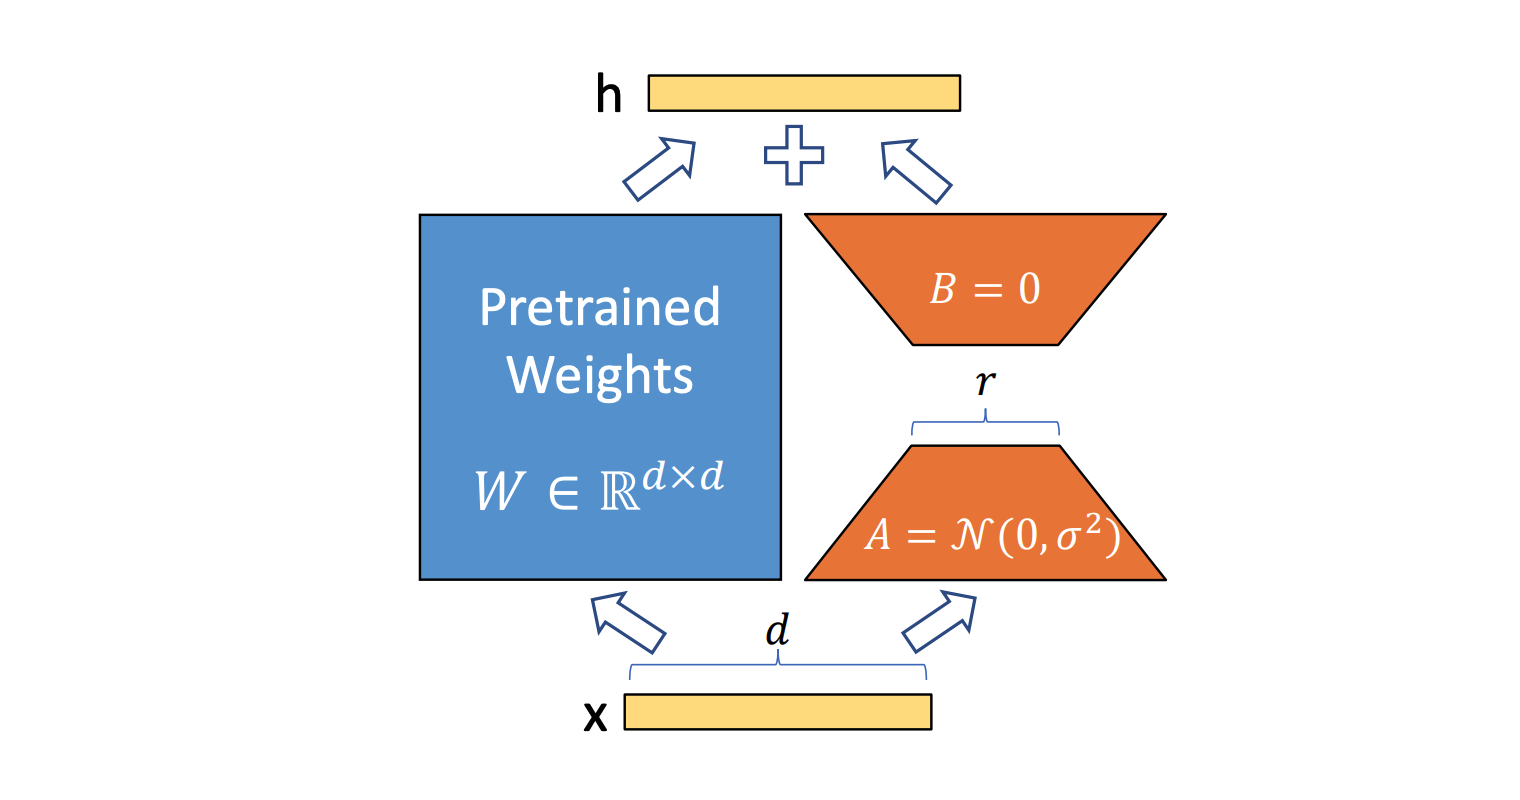
\includegraphics[width=0.6\linewidth,keepaspectratio]{lora1}
		
		{\tiny (Ref: https://heidloff.net/article/efficient-fine-tuning-lora/)}
		\end{center}

\end{frame}

%%%%%%%%%%%%%%%%%%%%%%%%%%%%%%%%%%%%%%%%%%%%%%%%%%%%%%%%%%%%%%%%%%%%%%%%%%%%%%%%%%
\begin{frame}[fragile]\frametitle{LoRA: Low-Rank Adaptation}
\begin{itemize}
    \item Introduces trainable rank decompositions of weight updates
    \item Instead of updating the full weight matrices, LoRA adds a small number of rank-decomposed weight matrices
    \item Significantly reduces the number of trainable parameters during fine-tuning
	\item As LoRA keeps original weights as is, it helps stopping catastrophic forgetting (new training, washing old learning)
\end{itemize}

		\begin{center}
		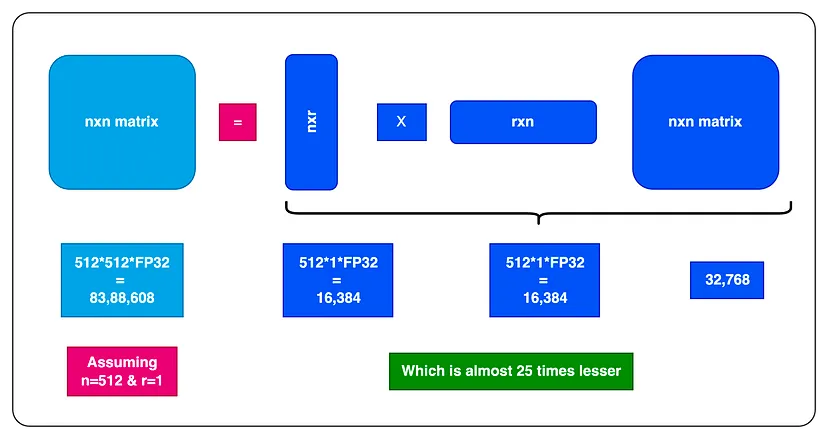
\includegraphics[width=0.6\linewidth,keepaspectratio]{lora2}
		
		{\tiny (Ref: https://abvijaykumar.medium.com/fine-tuning-llm-parameter-efficient-fine-tuning-peft-lora-qlora-part-1-571a472612c4)}
		\end{center}

\end{frame}


%%%%%%%%%%%%%%%%%%%%%%%%%%%%%%%%%%%%%%%%%%%%%%%%%%%%%%%%%%%%%%%%%%%%%%%%%%%%%%%%%%
\begin{frame}[fragile]\frametitle{LoRA: Low-Rank Adaptation}
    \begin{itemize}
        \item Pretrained original model weights are frozen
		\item Another set of weights are fine-tuned, meaning a difference-like-delta-weights are created such that when these deltas are added to original wrights, they act as if the combined model is tuned for the new corpus.
		\item So, have we doubled the parameters? original and fine-tuned sets? But that's on hard-disk. When we load it in GPU for inference, addition is done first and then loaded.
    \end{itemize}

		\begin{center}
		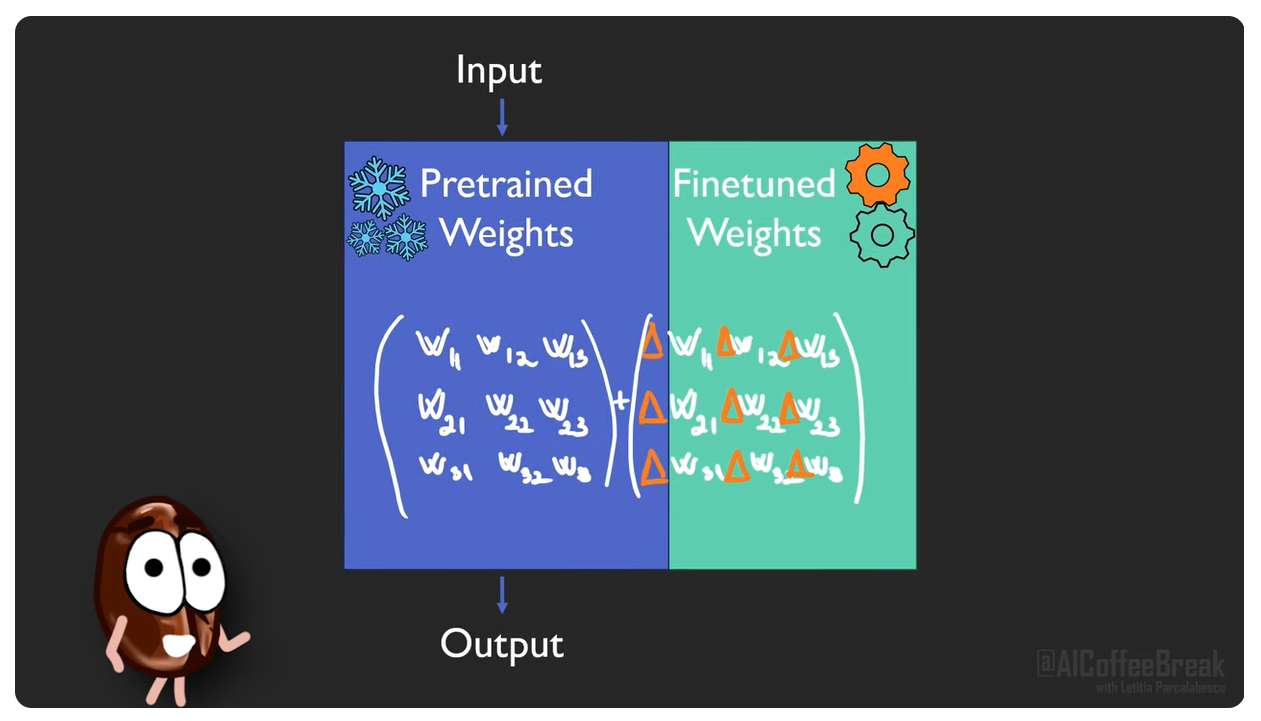
\includegraphics[width=0.5\linewidth,keepaspectratio]{lora4}
		
		{\tiny (Ref: What is LoRA? Low-Rank Adaptation for finetuning LLMs EXPLAINED-AI Coffee Break with Letitia)}
		\end{center}

\end{frame}

%%%%%%%%%%%%%%%%%%%%%%%%%%%%%%%%%%%%%%%%%%%%%%%%%%%%%%%%%%%%%%%%%%%%%%%%%%%%%%%%%%
\begin{frame}[fragile]\frametitle{LoRA: Low-Rank Adaptation}
    \begin{itemize}
        \item LoRA does a trick by which the number of fine-tuned weights are reduced.
		\item Leverages Rank of the matrix. In matrix, if some rows/columns are linearly dependent on others, they are redundant, as they can be generated by others. AFter such removal, the matrix dimension is the rank.
		\item So, just tune the weights of low rank, column and row vector.
		\item rank 'r' is the hyper parameter, we can chose.
		\item matrix 'A' is initialized from Gaussian distribution and 'B' with $0$ and let the back propagation, settle the weights.
    \end{itemize}

		\begin{center}
		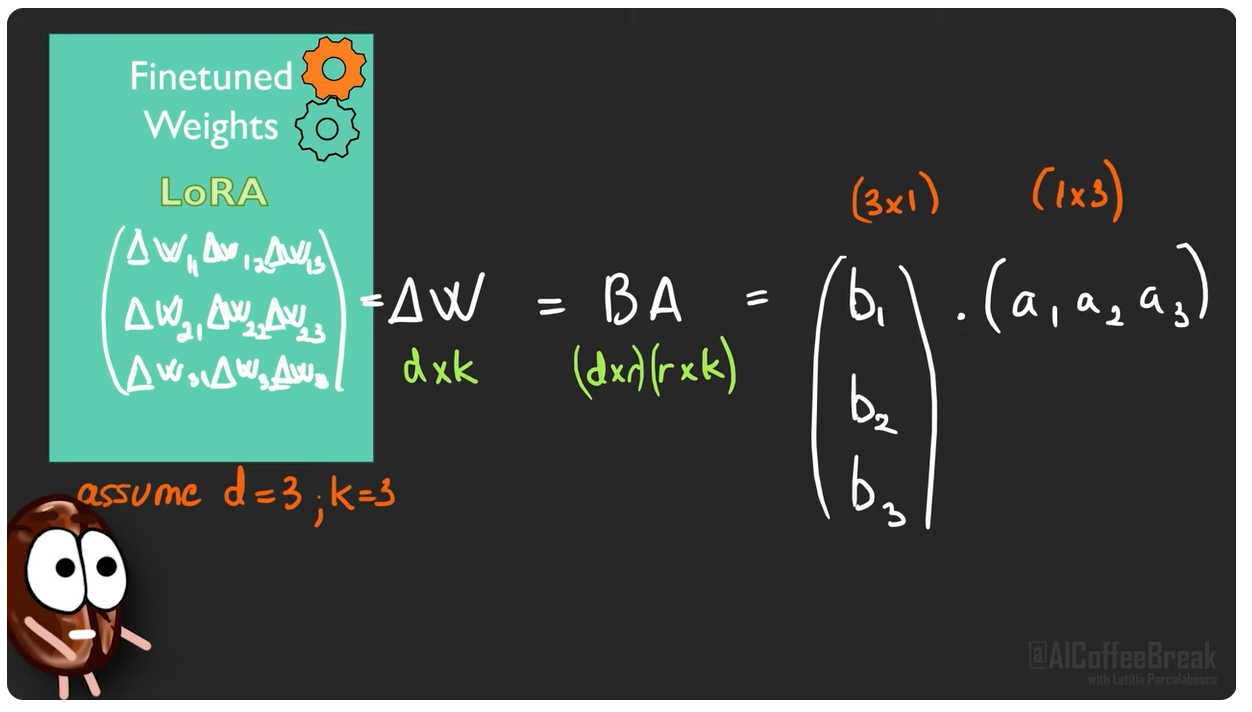
\includegraphics[width=0.5\linewidth,keepaspectratio]{lora5}
		
		{\tiny (Ref: What is LoRA? Low-Rank Adaptation for finetuning LLMs EXPLAINED-AI Coffee Break with Letitia)}
		\end{center}

\end{frame}



%%%%%%%%%%%%%%%%%%%%%%%%%%%%%%%%%%%%%%%%%%%%%%%%%%%%%%%%%%%%%%%%%%%%%%%%%%%%%%%%%%
\begin{frame}[fragile]\frametitle{LoRA: Low-Rank Adaptation}
    \begin{itemize}
        \item Original pre-trained parameters ($W$) are frozen
        \item New low-rank weight vectors $W_A$ and $W_B$ are added
        \item Dimensions: $W_A$ ($d \times r$), $W_B$ ($r \times d$), where $r < d$
        \item $r$ (rank) is a crucial parameter, lower $r$ means faster training but may impact performance
        \item Result computed as dot product of original and low-rank networks
        \item Loss function calculated, and $W_A$ and $W_B$ adjusted during backpropagation
    \end{itemize}

		\begin{center}
		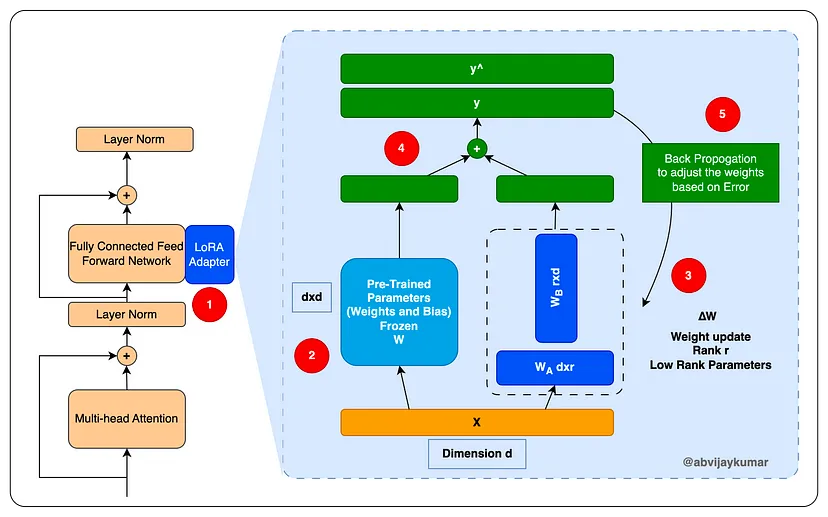
\includegraphics[width=0.5\linewidth,keepaspectratio]{lora3}
		
		{\tiny (Ref: https://abvijaykumar.medium.com/fine-tuning-llm-parameter-efficient-fine-tuning-peft-lora-qlora-part-1-571a472612c4)}
		\end{center}

\end{frame}


%%%%%%%%%%%%%%%%%%%%%%%%%%%%%%%%%%%%%%%%%%%%%%%%%%%%%%%%%%%%%%%%%%%%%%%%%%%%%%%%%%
\begin{frame}[fragile]\frametitle{LoRA Weight Update}
Let $W \in \mathbb{R}^{m \times n}$ be a weight matrix in the pre-trained LLM.
\begin{itemize}
    \item LoRA decomposes the weight update as $\Delta W = BA^T$
    \item $A \in \mathbb{R}^{r \times n}$ and $B \in \mathbb{R}^{m \times r}$ are trainable rank-$r$ matrices
    \item $r \ll \min(m, n)$, so the number of trainable parameters is greatly reduced
\end{itemize}
\end{frame}

%%%%%%%%%%%%%%%%%%%%%%%%%%%%%%%%%%%%%%%%%%%%%%%%%%%%%%%%%%%%%%%%%%%%%%%%%%%%%%%%%%
\begin{frame}[fragile]\frametitle{LoRA Training}
During fine-tuning, the weight matrix $W$ is updated as:
$$W' = W + \Delta W = W + BA^T$$
\begin{itemize}
    \item Only the low-rank matrices $A$ and $B$ are trained
    \item Pre-trained weights $W$ remain frozen
    \item Efficient memory-wise and compute-wise
\end{itemize}
\end{frame}

%%%%%%%%%%%%%%%%%%%%%%%%%%%%%%%%%%%%%%%%%%%%%%%%%%%%%%%%%%%%%%%%%%%%%%%%%%%%%%%%%%
\begin{frame}[fragile]\frametitle{LoRA Inference}
During inference, the updated weight matrix $W'$ is used:
$$W' = W + BA^T$$
\begin{itemize}
    \item No additional compute or memory required
    \item LoRA weight update is applied on-the-fly
\end{itemize}
\end{frame}


%%%%%%%%%%%%%%%%%%%%%%%%%%%%%%%%%%%%%%%%%%%%%%%%%%%%%%%%%%%%%%%%%%%%%%%%%%%%%%%%%%
\begin{frame}[fragile]\frametitle{LoRA: code}
\begin{lstlisting}
from transformers import AutoTokenizer, AutoModelForSeq2SeqLM
from peft import LoraConfig, get_peft_model, prepare_model_for_int8_training, TaskType

model = AutoModelForSeq2SeqLM.from_pretrained("google/flan-t5-xxl", load_in_8bit=True, device_map="auto")
lora_config = LoraConfig(
 r=16,
 lora_alpha=32,
 target_modules=["q", "v"],
 lora_dropout=0.05,
 bias="none",
 task_type=TaskType.SEQ_2_SEQ_LM
)
model = prepare_model_for_int8_training(model)
model = get_peft_model(model, lora_config)

model.print_trainable_parameters()
# trainable params: 18874368 || all params: 11154206720 || trainable%: 0.16921300163961817
\end{lstlisting}
\end{frame}


%%%%%%%%%%%%%%%%%%%%%%%%%%%%%%%%%%%%%%%%%%%%%%%%%%%%%%%%%%%%%%%%%%%%%%%%%%%%%%%%%%
\begin{frame}[fragile]\frametitle{What is QLoRA?}

  \begin{itemize}
    \item Memory-efficient iteration of LoRA.
    \item Quantizes weights of LoRA adapters to lower precision (e.g., 4-bit instead of 8-bit).
    \item Further reduces memory footprint and storage requirements.
    \item Pre-trained model loaded into GPU memory with quantized 4-bit weights.
    \item Despite reduction in bit precision, maintains comparable effectiveness to LoRA.
  \end{itemize}
  
  {\tiny (ref: Fine-Tuning LLMs : Overview, Methods, and Best Practices - Turing)}
  
\end{frame}

%%%%%%%%%%%%%%%%%%%%%%%%%%%%%%%%%%%%%%%%%%%%%%%%%%%%%%%%%%%%%%%%%%%%%%%%%%%%%%%%%%
\begin{frame}[fragile]\frametitle{}
\begin{center}
{\Large Summary}
\end{center}
\end{frame}

%%%%%%%%%%%%%%%%%%%%%%%%%%%%%%%%%%%%%%%%%%%%%%%%%%%%%%%%%%%%%%%%%%%%%%%%%%%%%%%%%%
\begin{frame}[fragile]\frametitle{Why Fine-Tune Large Language Models?}
  \begin{itemize}
    \item Adapt to specific tasks, domains, and nuances for enhanced performance. Fine-tuning for document analysis in the legal domain.
    \item Align models with new data distributions and out-of-distribution examples. Example: Fine-tuning a speech recognition model for a new regional accent.
    \item Transfer general knowledge from pre-trained models to specialized tasks. Example: Transferring medical knowledge to a healthcare chatbot.
    \item Optimize model parameters for task-specific objectives and user preferences. Example: Optimizing a pre-trained model for code generation in software development.
    \item Handle modest datasets and mitigate sub-optimal performance
    \item Bridges gap between general-purpose and specialized models.
    \item Enable continual learning and adaptation to evolving data and user needs.
    \item Improve factual responses and reduce hallucinations.
    \item Cost and resource efficiency compared to training from scratch.
  \end{itemize}
\end{frame}

%%%%%%%%%%%%%%%%%%%%%%%%%%%%%%%%%%%%%%%%%%%%%%%%%%%%%%%%%%%%%%%%%%%%%%%%%%%%%%%%%%
\begin{frame}[fragile]\frametitle{Advantages of PEFT}
  \begin{itemize}
    \item \textbf{Computational Efficiency:}
      \begin{itemize}
        \item PEFT fine-tunes LLMs with significantly fewer parameters than full fine-tuning.
        \item Feasible on less powerful hardware or in resource-constrained environments.
      \end{itemize}
    \item \textbf{Memory Efficiency:}
      \begin{itemize}
        \item Freezing pretrained model weights minimizes excessive memory usage.
        \item Suitable for tasks with memory constraints.
      \end{itemize}
    \item \textbf{Catastrophic Forgetting Mitigation:}
      \begin{itemize}
        \item PEFT prevents catastrophic forgetting observed in full fine-tuning.
        \item Ensures retention of valuable information during adaptation to new tasks.
      \end{itemize}
    \item \textbf{Versatility Across Modalities:}
      \begin{itemize}
        \item PEFT is effective in various modalities such as computer vision and audio.
        \item Applicable to a wide range of downstream tasks beyond natural language processing.
      \end{itemize}
  \end{itemize}
\end{frame}

%%%%%%%%%%%%%%%%%%%%%%%%%%%%%%%%%%%%%%%%%%%%%%%%%%%%%%%%%%%%%%%%%%%%%%%%%%%%%%%%%%
\begin{frame}[fragile]\frametitle{Advantages of PEFT (Contd.)}
  \begin{itemize}
    \item \textbf{Modular Adaptation for Multiple Tasks:}
      \begin{itemize}
        \item PEFT's modular nature allows the same pretrained model to be adapted for multiple tasks.
        \item Small task-specific weights are added, avoiding the need for full copies for different applications.
      \end{itemize}
    \item \textbf{INT8 Tuning:}
      \begin{itemize}
        \item PEFT includes INT8 (8-bit integer) tuning, showcasing adaptability to different quantization techniques.
        \item Enables fine-tuning even on platforms with limited computational resources.
      \end{itemize}
  \end{itemize}
\end{frame}

%%%%%%%%%%%%%%%%%%%%%%%%%%%%%%%%%%%%%%%%%%%%%%%%%%%%%%%%%%%%%%%%%%%%%%%%%%%%%%%%%%
\begin{frame}[fragile]\frametitle{Summary of PEFT}
  \begin{itemize}
    \item PEFT offers a \textbf{practical and efficient solution} for fine-tuning large language models.
    \item Addresses \textbf{computational and memory challenges} while maintaining performance on downstream tasks.
  \end{itemize}
\end{frame}

% %%%%%%%%%%%%%%%%%%%%%%%%%%%%%%%%%%%%%%%%%%%%%%%%%%%%%%%%%%%
% \begin{frame}[fragile]{Limitations of Fine-Tuning}
    % \begin{itemize}
        % \item Catastrophic Forgetting: Fine-tuned models may forget some aspects of their pre-trained knowledge as they adapt to the new task.
        % \item Computational requirements: Fine Tuning LLMs requires A100 GPU support.
        % \item Full Fine-Tuning learning parameter dimensions is equal to the pre-trained learning parameters
    % \end{itemize}
% \end{frame}



%%%%%%%%%%%%%%%%%%%%%%%%%%%%%%%%%%%%%%%%%%%%%%%%%%%%%%%%%%%%%%%%%%%%%%%%%%%%%%%%%%
\begin{frame}[fragile]\frametitle{LoRA Advantages}
\begin{itemize}
    \item Significantly reduces the number of trainable parameters
    \item Maintains performance comparable to full fine-tuning
    \item Efficient memory and compute usage
    \item Suitable for a wide range of tasks and models
    \item Allows fine-tuning on consumer-grade hardware
\end{itemize}
\end{frame}

%%%%%%%%%%%%%%%%%%%%%%%%%%%%%%%%%%%%%%%%%%%%%%%%%%%%%%%%%%%%%%%%%%%%%%%%%%%%%%%%%%
\begin{frame}[fragile]\frametitle{LoRA Limitations}
\begin{itemize}
    \item Performance may degrade for very low-rank approximations
    \item Potential for instability or divergence with extreme rank values
    \item May not be as effective for very small or very large models
    \item Requires careful tuning of rank and other hyperparameters
\end{itemize}
\end{frame}

% %%%%%%%%%%%%%%%%%%%%%%%%%%%%%%%%%%%%%%%%%%%%%%%%%%%%%%%%%%%%%%%%%%%%%%%%%%%%%%%%%%
% \begin{frame}[fragile]\frametitle{LoRA Variants and Extensions}
% \begin{itemize}
    % \item LoRA-UL: LoRA for Upsampling Layers
    % \item LoRA-Attention: LoRA for Attention Layers
    % \item LoRA-Dropout: LoRA with Dropout Regularization
    % \item LoRA-Distillation: Knowledge Distillation with LoRA
    % \item LoRA-Composition: Composing LoRA with other Techniques
% \end{itemize}
% \end{frame}



%%%%%%%%%%%%%%%%%%%%%%%%%%%%%%%%%%%%%%%%%%%%%%%%%%%%%%%%%%%%%%%%%%%%%%%%%%%%%%%%%%
\begin{frame}[fragile]\frametitle{Summary of LoRA}

\begin{itemize}
    \item LoRA is an efficient fine-tuning technique for large language models
    \item Reduces computational cost while maintaining performance
    \item Enables fine-tuning on consumer-grade hardware
    \item Applicable to various tasks and models
    \item Active area of research with ongoing improvements and extensions
\end{itemize}
\end{frame}


